\clearpage
\twocolumn[{%
\subsection{Evaluation recipe}
\label{app:rq11_evaluation_recipe}

\noindent\begin{minipage}[t]{0.485\textwidth}
\vspace{0pt}
\paragraph{Research Question.} \emph{The rest of the analysis asks whether a cheap measurement reproduces the 1.7B reference's design decision. This analysis turns that into advice for a reader who has to choose what to evaluate: for each benchmark, which \textbf{variant} (the items as published, their \texttt{rf\_} cloze rewrite (RF) or their \texttt{rfgm\_} LLM rewrite (LLM-RF), scored by \textbf{accuracy} or by the gold answer's \textbf{bits per byte} (bBPB)) reads the reference's decision from the smallest proxy?}

\paragraph{Setup.} Seed-1904 runs of every cell. We report the DA-size of the proxies 90M--1B against the 1.7B final checkpoint, on multi-axis pairs and on the tasks above chance at the proxy and at the reference. Each benchmark is read in up to six ways. The items are used as published, as RF or as LLM-RF, and each version is scored by accuracy or by the bits per byte of the gold answer (bBPB).
\end{minipage}\hfill
\begin{minipage}[t]{0.485\textwidth}
\vspace{0pt}
\begin{rqfinding}
\textbf{1. No way of evaluating a benchmark reads the reference's accuracy decision at $\tau$ = 0.75 on average at any proxy up to 1B.} The best mean is 0.63 (LLM-RF bBPB at 90M, only the easier bBPB $\rightarrow$ 1.7B bBPB target, LLM-RF at 0.71--0.80, clears it). Against the same truth, bBPB matches or edges the original accuracy at all five proxies (every task: 0.59--0.61 against 0.55--0.60, paired: 0.60--0.64), and the rewrites help only when scored by bBPB (RF and LLM-RF accuracy 0.48--0.56 across the five proxies, their bBPB 0.57--0.63). (Figure~\ref{fig:app_rq11_evaluation_recipe}.)
\\
\\
\textbf{2. Against the same truth (bBPB $\rightarrow$ 1.7B accuracy), bBPB is the pick for 17 of the 23 benchmarks with a value and accuracy for 6.} (8 of 31 have none).
\\
\\
\textbf{3. The pick is now like for like.} A bBPB task is ranked on the same five proxies as an accuracy task.
\end{rqfinding}
\end{minipage}

\vspace{\baselineskip}
\noindent\begin{minipage}{\textwidth}
\centering
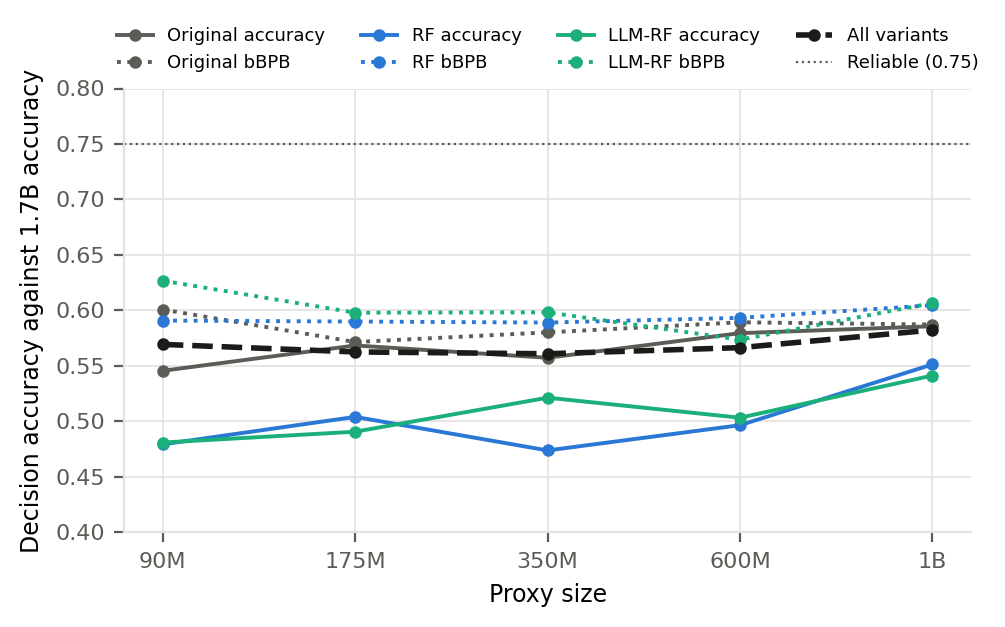
\includegraphics[width=\textwidth,height=0.4\textheight,keepaspectratio]{figures/app_rq11_evaluation_recipe.png}
% source: src/signal-and-noise/analysis/rq11_evaluation_recipe/pretraining/predictivity/recipe_da_size_variants_multi_axes_paper.png
\captionof{figure}{\textbf{No way of evaluating a benchmark reads the reference's accuracy decision at $\tau$ = 0.75 on average at any proxy up to 1B.} Mean DA-size against the 1.7B accuracy for each way of reading a benchmark, by proxy size. The colour gives the item format (original, RF, LLM-RF) and the line style the score (solid for accuracy, dotted for bBPB). The dashed black line pools every variant and the dotted line marks 0.75.}
\label{fig:app_rq11_evaluation_recipe}
\end{minipage}
\vspace{\baselineskip}
}]
